%%%%%%%%%%%%%%%%%%%%%%% file template.tex %%%%%%%%%%%%%%%%%%%%%%%%%
%
% This is a general template file for the LaTeX package SVJour3
% for Springer journals.          Springer Heidelberg 2010/09/16
%
% Copy it to a new file with a new name and use it as the basis
% for your article. Delete % signs as needed.
%
% This template includes a few options for different layouts and
% content for various journals. Please consult a previous issue of
% your journal as needed.
%
%%%%%%%%%%%%%%%%%%%%%%%%%%%%%%%%%%%%%%%%%%%%%%%%%%%%%%%%%%%%%%%%%%%
\begin{filecontents*}{example.eps}
%!PS-Adobe-3.0 EPSF-3.0
%%BoundingBox: 19 19 221 221
%%CreationDate: Mon Sep 29 1997
%%Creator: programmed by hand (JK)
%%EndComments
gsave
newpath
  20 20 moveto
  20 220 lineto
  220 220 lineto
  220 20 lineto
closepath
2 setlinewidth
gsave
  .4 setgray fill
grestore
stroke
grestore
\end{filecontents*}
%
\RequirePackage{fix-cm}
%
\documentclass{svjour3}                     % onecolumn (standard format)
%\documentclass[smallcondensed]{svjour3}     % onecolumn (ditto)
%\documentclass[smallextended]{svjour3}       % onecolumn (second format)
%\documentclass[twocolumn]{svjour3}          % twocolumn
%
\smartqed  % flush right qed marks, e.g. at end of proof
\usepackage{graphicx}
\usepackage{cite}
\journalname{Requirements Engineering}
\begin{document}

\title{Network Structure and the Effectiveness of Crowd-Based Requirements Processes}
\titlerunning{Network Structure and the Effectiveness of Crowd-Based Requirements Processes}

\author{Matthew Robinson \and
        Shahram Sarkani \and 
        Thomas Mazzuchi
}

\authorrunning{Robinson, Sarkani, and Mazzuchi} % if too long for running head
\institute{M. Robinson \at \email{mrobinson23@gwu.edu}}

\date{Received: date / Accepted: date}
% The correct dates will be entered by the editor


\maketitle

\begin{abstract}
Systems engineering researchers have argued that crowd-sourcing generates better requirements by eliciting feedback from a broader range of stakeholders. Proposed benefits of crowd-based requirements processes include a higher volume of requirements reflecting a more comprehensive array of use cases and a more engaged and committed user base. Researchers cite the inability of project teams to effectively manage an overwhelming volume of crowd-sourced system requirements as a possible drawback. This paper analyzes a data set consisting of project management artifacts from 562 open-source software projects using generalized linear models to determine how system performance varies as the percentage of requirements sourced from the crowd increases for five measures of effectiveness: requirement close-out time, requirement response time, comment activity, the average number of issues per crowd member, and the volume of requirements over time. Additionally, the models measure how the impact of additional crowd engagement changes with stakeholder network structure. The analysis shows that stakeholder network structure and the level of crowd-sourcing impact each measure of effectiveness except issues per user. The results imply stakeholder networks with multiple, disjoint hubs and a low level of localized clustering absorb additional crowd engagement most effectively and suggest that systems engineers who seek to employ crowd-based requirements processes should encourage specialization amongst contributors and develop procedures to route incoming requirements to the appropriate specialist. Moreover, increased crowd-sourcing is most beneficial to projects that current source small to moderate share of requirements from the crowd. 
\keywords{Crowd-Based Requirements Engineering \and Stakeholder Networks \and Network Analysis \and Stakeholder Analysis \and Generalized Linear Models}
\end{abstract}

\section{Introduction}
\label{intro}

The growing prevalence of systems with diverse and distributed stakeholders has stretched the limits of traditional stakeholder analysis techniques. These conditions make it difficult for systems engineers to identify an exhaustive list of stakeholders at the onset of a project. The consequent uncertainty during the stakeholder analysis process can negatively impact the quality of system requirements. To deal with this challenge, researchers have begun to develop techniques, known as crowd-based requirements processes, to facilitate crowd-sourcing requirements from users.

Advocates of crowd-based requirements processes argue that engaging with crowds enables systems engineers to understand the range of potential use cases for a system more fully \cite{groen}. Improved understanding of stakeholder needs translates into better system requirements and more informed prioritization decisions. Crowd-sourcing, however, also has drawbacks. A high volume of requirements can overwhelm engineers and project managers, and some experts have questioned the quality of crowd-sourced requirements \cite{snijders}. Systems engineers need to consciously evaluate these trade-offs before determining the extent to which they will rely on crowd-sourcing during the requirements process. Moreover, systems engineers need a framework for assessing whether or not they should encourage more crowd-sourcing, given the current state of the system.

Network analysis provides a useful framework for thinking about and measuring patterns of interaction between crowd members and project contributors. Systems engineers can model crowd-contributor interactions as a stakeholder network, where nodes represent stakeholders, and edges represent collaboration between stakeholders on the same requirement. This research asserts that the structure of the stakeholder network influences the effectiveness of crowd-based requirements processes and employs regression analysis to test this claim empirically for five measures of effectiveness: requirement close-out time, requirement response time, comment activity, the number of requirements per crowd member, and the volume of requirements over time.

Analysis based on a curated set of 562 open-source software projects on GitHub demonstrates that stakeholder network structure has a statistically significant impact on each measure of effectiveness except for the number of requirements per crowd member. The data suggest that stakeholder networks with multiple, disjoint hubs and low localized clustering absorb additional crowd-sourcing most effectively. Systems that already source a low-to-moderate number of requirements from the crowd benefit the most from increased crowd-sourcing. For systems that crowd-source more than 60-65\% of requirements, the downsides of additional crowd-sourcing outweigh the benefits. From a practical standpoint, the analysis implies that systems benefit most from crowd-sourcing when they have the following characteristics:

\begin{itemize}
    \item Multiple contributors who specialize in a distinct component of the system
    \item A process for assigning the requirements to the proper contributor
    \item Direct interaction between crowd-members and contributors
    \item Minimal interaction between crowd-members
\end{itemize}

Since the data set consists of widely adopted open-source software packages, readers should apply caution before generalizing these results to other domains. Physical products, proprietary software, and even smaller open-source software projects face different challenges, which may favor stakeholder networks with different structures.

This paper begins by reviewing the literature on crowd-based requirements processes, stakeholder networks, and open-source software systems. The methodology section details the data set, explains the experimental design, justifies each modeling decision, and highlights potential drawbacks. The results section presents the regression models and associated diagnostics. The paper concludes by interpreting the results, discussing limitations, and suggesting avenues for future research.

\section{Literature Review}
\label{litreview}

\subsection{Crowd-Based Requirements Processes}
\label{crowd_based_re}
In his seminal work on the topic, Howe describes crowd-sourcing as the process of outsourcing tasks to a network of contributors through an open call for participation \cite{howe, howe2}. As early as 2002, Finkelstein anticipated the importance of crowd-sourcing for requirements engineering, despite, at the time, the lack of platforms that could facilitate distributed, asynchronous collaboration on projects \cite{finkelstein}. With the emergence of adequate tools, crowd-sourcing has grown more prevalent, particularly in the field of software engineering. According to Mao, Capra, Harman, and Jia, published research on crowd-sourcing within the software engineering domain grew from only one paper in 2008 to over 200 in 2015 \cite{mao}. Writing in 2015, LaToza and Van Der Hoek note the rise of several crowd-sourcing modalities within the software engineering community, including peer participation, competitions, and micro-tasking \cite{latoza}. Treatment of the topic within the context of software engineering, however, has primarily focused on implementation. Although Stol, LaToza, and Bird argue that crowd-sourcing facilitates quicker identification of bugs and more productive feedback \cite{stol}, they do not discuss the implication of these outcomes for stakeholder analysis more broadly.
 
By contrast, the requirements engineering literature features a lively discussion of how crowd-sourcing intersects with stakeholder analysis. Gerth, Burnap, and Papalambros provide a survey of the topic and highlight both the benefits and challenges of crowd-sourcing. They argue that while crowd-sourcing can improve the quality of requirements under the right circumstances, crowd-sourcing only produces these benefits if systems engineers institute well-governed processes for managing the crowd. Optimizing these processes presents challenges for systems engineers because different use cases and crowd sizes demand different approaches \cite{gerth}.

The requirements engineering community has spent considerable effort to develop tools and processes for effectively managing crowds. In addition to proposing solutions, this literature contains ample discussion about the drawbacks of crowd-sourcing. Finkelstein and his colleagues developed software packages such as StakeRare and StakeNet to address concerns about the ability of systems engineers to prioritize requirements effectively when faced with an overwhelming volume of feedback from the crowd \cite{stakerare, stakenet}. Their network-based approach uses centrality measures to identify the most influential stakeholders in the system and allows project managers to prioritize requirements accordingly \cite{lim}. Finkelstein and his colleagues claim crowd-based requirements processes enable systems engineers to discover use cases and stakeholders that they failed to identify during the system design phase \cite{stakerare}. By engaging with crowds early in the utilization process, systems engineers can iterate on the design and avoid investment in solutions that do not truly address stakeholder needs. Groen highlights potential drawbacks to this approach, including a tendency for systems engineers to overlook the needs of critical stakeholders who engage less actively with the rest of the network \cite{groen}.

Other researchers have sought to allay concerns about the motivation of crowd members and their willingness to remain engaged in the requirements process over time. Groen, Dalpiaz, Ali, and their colleagues insist that crowd members need an incentive to produce high-quality requirements \cite{groen}. Snijders and Dalpiaz develop a solution based on gamification, in which systems engineers offer explicit rewards to induce crowd members to remain engaged \cite{snijders, snijders2}. Hosseini, Phalp, Taylor, and Ali assess that properly incentivizing crowd members produces a host of benefits, including an improved ability to adapt requirements to changing conditions, empirical validation of assumptions about the system, and the identification of new stakeholders and use cases \cite{hosseini}. These advantages accrue most readily to systems that contend with more uncertainty.

Levy, Hadar, and Te'eni agree that crowd motivation presents a risk. They propose an alternative solution to mitigate it based on what they call micro-crowds \cite{levy}. In the early stages of a project, their strategy calls for the development of smaller, more cohesive micro-crowds based on the theory that crowd members have a higher probability of remaining engaged if they form strong bonds with fellow participants. As a project expands, systems engineers work to connect independent micro-crowds and establish a broader community. The micro-crowds approach empowers systems engineers to encourage connections that benefit the system as a whole, rather than merely relying on the organic behavior of the crowd. By starting small and ensuring contributors remain actively engaged, the micro-crowd approach aims to increase user satisfaction and produce higher quality requirements for the system.

\subsection{Network Analysis in Requirements Engineering}
\label{network_re}

In recent years, the research community has also expressed interest in quantifying how stakeholder network structure affects the requirements process. Several methodologies have emerged that use network analysis to identify core and peripheral stakeholders, a distinction that arises from Newcombe's observation that stakeholders with varying degrees of involvement can influence the priorities of a project \cite{newcombe}. Missonier and Loufrani-Fedida developed an approach based on actor-network theory, which describes stakeholder networks as dynamic social constructs whose characteristics and effectiveness change over time \cite{missonier}. Wood, Sarkani, Mazzuchi, and Eveleigh operationalize this concept and construct network maps using crosswalks that connect stakeholders with common interests in a system component \cite{wood}. In their pilot study, they use project management artifacts to identify relationships between stakeholders. 

Other research has focused on how network structure influences dynamics within a project. Linaker, Regnell, and Damian, for instance, show that stakeholders who occupy central positions within a network more strongly influence the priorities of open-source software projects \cite{linaker}. Separately, Damian, Marczak, and Kwan use social networks to show that physical distance does not limit the ability of remote software development teams to collaborate effectively on requirements \cite{damian}. Toral, Martinez-Torres and Barrero study how network concentration affects the level of engagement on discussion threads related to the open-source Linux operating system \cite{toral}. Their research shows that higher network concentration improves the flow of information within the community because key contributors act as knowledge brokers who help to connect disparate sub-communities. However, they also note that excessive concentration presents barriers to the integration of new community members, and can lead the community to rely on a small number of core contributors.

Another category of research evaluates the relative effectiveness of different stakeholder network topologies. Iyer and Lyytinen show that, in general, open-source software projects with more centralized communications structures have higher task completion rates \cite{iyer}. The advantage of centralizing, however, diminishes as requirement volume increases. For projects that contend with a high volume of requirements, they recommend decentralized project management processes. In addition to developing robust methodologies for constructing stakeholder networks, the studies outlined in this section inform initial expectations about how network structure will affect system performance.

\subsection{Research Gap}

This research extends the literature by empirically evaluating how stakeholder networks with different structures perform when they crowd-source requirements. While Iyer and Lyytinen compare effectiveness across network structures, their study does not consider the level of crowd-sourcing. Furthermore, their work focuses on network concentration and task completion rate but does not evaluate other network topology measures or project management measures of effectiveness. Separately, Groen and his colleague cite the sparsity of empirical research on crowd-based requirements processes as a significant concern \cite{groen}, making this a particularly useful contribution to the literature on crowd-based requirements processes. Overall, this research seeks to assess the validity of theoretical claims about crowd-based requirements engineering and study the interaction between network structure and crowd-sourcing. The results will enable systems engineers to answer the question: Given the structure of the stakeholder network for my system and the current level of crowd-sourcing, should I encourage additional engagement with the crowd?

\section{Methodology}

To evaluate how the effectiveness of crowd-sourcing changes with network structure, the research team employs the following procedure:

\begin{enumerate}
    \item Build stakeholder networks from project management data.
    \item Measure the intensity of crowd-sourcing for each project.
    \item Train regression models to estimate the effect of crowd sourcing and stakeholder network structure.
    \item Interpret the results.
\end{enumerate}

The methodology section begins with a detailed description of the data set and then defines the input variables for the regression models. Inputs to the regression models include the percentage of crowd-sourced requirements, network structure variables, the project management measures of effectiveness, and several control variables. Finally, the section outlines the statistical analysis framework, which utilizes generalized linear models.

\subsection{Data Set}
\label{data_set_section}

This research leverages publicly available project management data from GitHub, a widely used code repository and collaboration tool. In total, the data set consists of 562 packages from a curated set of open-source projects and includes information about 24,730 distinct users, 34,982 issues, and about 165,836 comments. The curated list of projects originated from community maintained repositories containing links to popular packages for the five most commonly used programming languages: C++, Java, JavaScript, PHP, and Python  \cite{cpp, java, javascript, php, python}. The research team used the GitHub application programming interface in June 2019 to download project management data for each project. Since the analysis depends on having enough information to build a meaningful stakeholder network, the data set only includes projects that have at least thirty requirements.

Stakeholders in a GitHub project fall into two categories: contributors and users. Contributors include any stakeholder who has committed code to a project. By contrast, users do not write source code for a project but participate in the software development process by providing feedback and submitting requirements, thus making them stakeholders in the requirements engineering process according to Sharp and Finkelstein's definition \cite{sharp}. Note, not every user submits system requirements. As a result, the data set reflects the activity of the most engaged subset of users. Within the data set, any requirement originating from a non-contributor counts as a crowd-sourced requirement.

GitHub projects manage requirements through issues. Collaboration on issues occurs through comments. Issues and comments also serve as documentation. GitHub tracks both tasks and pull requests as issues. The analysis excludes pull requests because pull requests reflect contributions to the code base rather than requirements. GitHub issues present additional difficulty because, in some cases, issues function as a help forum rather than a project management artifact. Fortunately, GitHub provides labels to separate questions from tasks. To limit the analysis to project requirements, the data only includes issues with the labels “bug”, “change”, “enhancement”, “feature”, “feature request”, or “suggestion” and ignores issues with the labels “documentation”, “help wanted”, and “question”. Although GitHub allows users to create custom labels, the analysis discards them because most custom labels appear in only a single project.

\subsection{Crowd-source Percentage}

The percentage of crowd-sourced requirements measures the intensity of crowd-sourcing for a project and, in addition to network structure, represents the primary variable of interest. Computing this variable involves counting the number of crowd-sourced requirements as defined in Section \ref{data_set_section} and dividing that by the total number of requirements. Since some code contributions come from developers who do not belong to the core project team, this definition undercounts the number of crowd-sourced requirements, but probably not by a considerable margin. Undercounting would only present a concern if requirements from non-core contributors constituted a large percentage of crowd-sourced requirements, which in most cases they do not.  A histogram of crowd-source percentage appears in Figure \ref{crowd_pct_hist} and reveals an approximately uniform distribution across the entire range of values. The wide distribution of crowd-source percentage underscores the diversity of project management strategies for open-source projects and makes the data set ideal for comparing their relative effectiveness.

\begin{figure*}
  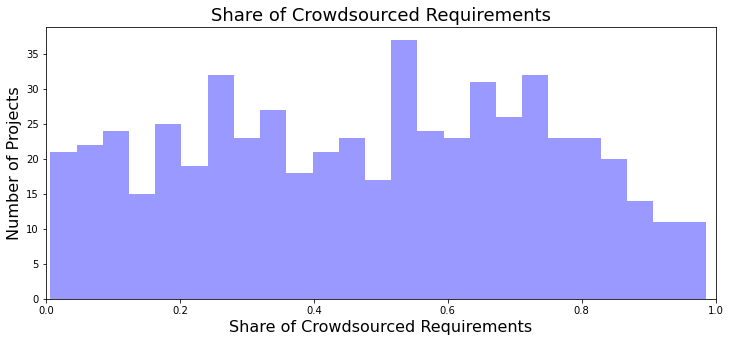
\includegraphics[width=0.95\textwidth]{crowd_pct_hist.png}
\caption{Percentage of crowd-sourced requirements in the data set.}
\label{crowd_pct_hist}
\end{figure*}

\subsection{Network Analysis}

Analyzing how the effectiveness of crowd-sourcing changes with network structure requires a strategy for constructing stakeholder networks from GitHub data and measuring the structure of those networks. This subsection covers both of those procedures in detail.

\subsubsection{Constructing Networks}
\label{network_section}

The stakeholder networks in this study consist of undirected, unweighted graphs where nodes represent stakeholders and edges represent collaboration on a requirement. As noted in Section \ref{data_set_section}, the stakeholders in the data set only include contributors and users who have submitted requirements. Using the definition from Mitchell, Agle, and Wood, this constitutes a narrow stakeholder set because it excludes stakeholders who do not directly participate in the requirements process \cite{mitchell}. Of course, concentric circles of stakeholders exist beyond this core group, including users who have not submitted requirements, developers of dependent packages, and the broader community for a programming language. Since this study focuses on the requirements process, excluding peripheral stakeholders does not materially affect our results.

Using undirected, unweighted graphs follows a pattern established in most of the studies cited in Section \ref{network_re}. Weighted edges provide an advantage insofar as they allow the model to capture the intensity of the relationship between stakeholders. Toral, Martinez-Torres, and Barrero, for instance, use weighted edges to study the influence of knowledge brokers within networks and argue that more frequent interactions indicates a more robust connection between stakeholders \cite{toral}. The network models in this research do not include weights because, for some metrics, their inclusion produces counter-intuitive results. Higher edge weights, for instance, typically reflect longer distances between nodes, whereas more frequent interactions should reduce the distance between stakeholders. Edge weights do improve fidelity for centrality measures, such as the edge degree of nodes. However, weighting would also reduce the variability of concentration measurements within the data set, making statistical inference more difficult. Given the methodological difficulty involved in incorporating edge weights and the limited potential benefit, the research team decided to use unweighted edges.

Toral, Martinez-Torres, and Barrero use directed edges to represent information flow within their networks \cite{toral}. Specifically, they use discussion threads as the primary unit of analysis and construct networks that represent a directed chain of replies. Within the context of their work, directed edges add value due to their ability to model information flows. In the current study, however, networks represent two-way collaborations rather than a series of replies, meaning undirected edges have a more intuitive interpretation. As a result, the research team decided to construct the stakeholder networks using undirected edges.

\subsubsection{Measuring Network Structure}
\label{network_structure}

Network structure measures include the Gini coefficient for network concentration, average minimum path for network breadth, and the clustering coefficient for the level of localized clustering. These numerical measures produce more information than categorical measures of network structure and make the resulting models more intuitive for the systems engineering use case. Systems engineers do not have enough control over a stakeholder network to change its structure from one broad category to another. However, they can implement strategies that nudge the structure of the network in one direction or another. As a result, systems engineers benefit more from an understanding of the impact of smaller changes in network structure. Numerical measures capture these changes better than categorical variables.

The Gini coefficient measures the amount of inequality in the degree distribution of the nodes and characterizes the level of concentration in the network. The measure ranges from zero to one. Zero reflects perfects equality and one represents perfect inequality \cite{gini}. Although typically applied in the context of income inequality \cite{gini2, yitzhaki}, Toral, Martinez-Torres, and Barrero show that the Gini coefficient also provides a useful measure of concentration in contributor networks for open-source software \cite{toral} . 

Note, the value of the Gini coefficient for the degree distribution of nodes in a network cannot reach one because every edge connects to a pair of nodes. As a result, a single node cannot collect degrees without sharing degrees with other nodes. As a result, the maximum value for the Gini coefficient for a network grows with the number of nodes, but never reaches one. Similarly, the effective lower bound of the Gini coefficient for networks remains above zero. Although this property makes the Gini coefficient an imperfect measure of network concentration, as a practical matter, it only impacts relatively small networks.

The original formulation defines the Gini coefficient using the Lorenz curve \cite{gini}. However, Sen provides an equivalent formulation, which calculates the Gini coefficient as half the mean absolute difference \cite{sen}. This formulation appears in Equation \ref{gini_coef}. Due to its simplicity, the research team decided to compute the Gini coefficient using the Sen formulation.

\begin{equation}
\label{gini_coef}
    G = \frac{\sum_{i=1}^{n} \sum_{j=i}^{n} | x_{i} - x{j} |}{2n^2 \bar{x}}
\end{equation}

The average minimum path measures the dispersal of the network. Computing this metric involves finding the minimum path between each pair of nodes in the network and taking the simple mean of the resulting minimum paths. The clustering coefficient, which calculates the probability that two incident nodes will form a triangle and takes values between zero and one, serves as a measure of the degree of localized clustering in a network \cite{holland}. Networks with a low level of localized clustering have hub-and-spoke structures, whereas networks with substantial localized clustering look more like webs.

Watts and Strogatz describe networks with low average minimum paths and low localized clustering as small-world networks \cite{watts}. In small-world networks, hubs tend to form, which serve as connectors between more remote nodes. By contrast, a high average minimum path combined with high localized clustering would indicate a distributed network with frequent collaboration between stakeholders in different parts of the network. Section \ref{results_section} includes a discussion of the relative effectiveness of these different network configurations.

To capture how the effectiveness of crowd-sourcing changes with network structure, the models also include interaction terms between each network structure variable and the percentage of crowd-sourced requirements. Interpreting the coefficients on these variables enables systems engineers to determine under what conditions they should consider promoting additional crowd-sourcing. Moreover, a dependent relationship exists between the three network structure variables because, for instance, a change in network concentration could also change the breadth of the network. To capture this relationship, the regression models include interaction terms between the network structure variables in cases where those terms have statistically significance and materially improve the fit of the model.

\subsection{Measures of Effectiveness}
\label{measures_of_effectiveness}

While not exhaustive, the analysis targets measures of effectiveness related to the proposed advantages and disadvantages of crowd-based requirements processes. Each measure of effectiveness derives from the existing literature on the topic. The measures of effectiveness considered as dependent variables in the analysis include:

\begin{itemize}
    \item The average requirement close-out time
    \item The average response time to a new requirement
    \item The average number of comments on each requirement
    \item The number of issues per user
    \item The volume of requirements
\end{itemize}

The first two metrics relate to a concern that Snijders and his colleagues raise. Namely, they worry that members of the crowd will lose interest if project teams do not address their requirements quickly \cite{snijders, snijders2}. Higher performing teams respond to and implement requirements more quickly. Project teams closeout a requirement when they either (a) implement the requirement or (b) decide not to address it. Since either outcome provides feedback to the crowd member who submitted the issue, both reflect strong engagement from the project team. Average close-out time computes the mean difference in days between the issue submission time and the last response time on the issue from the project team. The computation for this metric only includes requirements that the project team has closed. The final response time from the project team produces a more accurate estimate of the active time for the requirement than time to closure because engineering teams often do not close issues until they release a version of the package that includes the new feature. The average response time measures the mean number of days between the issue submission time and the first response from the project team. Lower values for average close-out time and response time reflect positive outcomes.

Other purported benefits of crowd-based requirements processes include higher quality requirements \cite{hosseini} and a more motivated and active user base \cite{groen}. While challenging to measure directly, the average number of comments per issue serves as a proxy for requirement quality. More comments indicate a requirement has garnered more interest, which suggests higher quality content. As noted in Toral, Martinez-Torres, and Barrero, threaded discussions require participants to commit more cognitive resources and indicate a higher level of engagement \cite{toral}. The number of issues per user measures engagement more directly. A higher number of issues per user mean crowd members have returned to submit multiple requirements and remain continuously engaged with the project. For both of these variables, higher values represent positive outcomes.

Increasing the volume of requirements can represent either a positive or a negative outcome, depending on the context. On the one hand, a higher volume of requirements enables systems engineers to process feedback from a broader range of stakeholders \cite{hosseini}. However, an excessive number of requirements can overwhelm project teams and make prioritization difficult \cite{groen, stakenet, stakerare}. Therefore, issue volume requires additional context from the other variables to determine whether it helps or hurts.

Although these measures of effectiveness cover many of the proposed benefits and challenges of crowd-sourcing, several remain unaddressed. Hosseini claims that crowd-sourcing enables systems engineers to discover use cases they did not anticipate during the design phase \cite{hosseini}. Since the GitHub data set does not contain any information from the design phase, this remains outside the scope of the analysis. Additionally, this study does not address the prioritization of individual requirements. Lim and his colleagues identify a tendency for systems engineers to overlook the needs of potentially relevant stakeholders who do not actively engage in public forums as a potential adverse side effect of crowd-sourcing \cite{stakenet}. The GitHub data set makes it difficult to infer the relative prioritization of requirements due to ambiguity about whether a project team has implemented or dismissed a requirement. While strategies exist to address this issue---for instance, searching for linked pull requests---the research team kept prioritization of individual requirements out of scope due to their complexity.

\subsection{Control Variables}

\subsubsection{Derived Variables}

While not primary variables of interest, the analysis includes project age, the number of contributors, the number of crowd participants, and the number of issues as control variables to improve inference. As shown in Figure \ref{feature_histograms}, the number of crowd participants, the number of contributors, and the number of issues each have left-skewed distributions with long right tails. By contrast, the age of the projects in the data set has an approximately normal distribution, with ages ranging from slightly over one year to almost sixteen years. Summary statistics for each of these variables appear in Figure \ref{feature_histograms}.

\begin{table}
\caption{Summary Statistics for Independent Variables}
\label{iv_summary}
\begin{tabular}{llllll}
\hline\noalign{\smallskip}
Variable & Min & 25\% & Median & 75\% & Max  \\
\noalign{\smallskip}\hline\noalign{\smallskip}
Project Age & 1.24 & 4.24  & 5.51 & 6.87 & 15.63 \\
Contributors & 1 & 5 & 9 & 15 & 86 \\
Crowd Participants & 1 & 14 & 24 & 42 & 311 \\
Issues & 30 & 48 & 77 & 142 & 1660 \\
\noalign{\smallskip}\hline
\end{tabular}
\end{table}

\begin{figure*}
  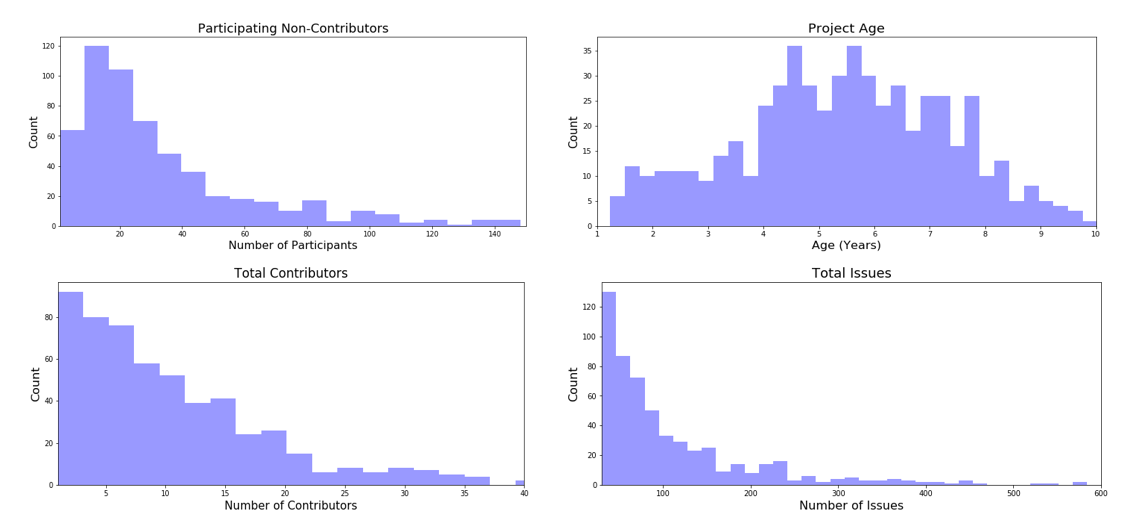
\includegraphics[width=0.95\textwidth]{feature_histograms.PNG}
\caption{Histograms for explanatory variables.}
\label{feature_histograms}
\end{figure*}

\subsubsection{Topic Variables}
\label{topic_modeling}

In addition to simple derived variables, the analysis includes control variables that capture qualitative information about the requirements for each project. Constructing these variables involves training a topic model on the content of the requirements in the data set. The complexity of a requirement substantially impacts the level of engagement needed from the project team. As a result, the research team assessed that the potential benefits of these variables justified the additional model complexity.

The topic model converts the text description of each requirement to a numerical vector using term frequency-inverse document frequency (TF-IDF). TF-IDF determines the importance of a word by counting the number of times it appears in a requirement, and scales it by the number of times it appears in the full corpus \cite{aizawa}. The TF-IDF vectors for each requirement combined to form the input matrix for a Latent Dirichlet Allocation (LDA) model. LDA treats the distribution of topics in the requirement set as a Dirichlet distribution over a fixed number of topics. For each requirement, LDA assigns a probability for each topic based on the text of the requirement \cite{blei}. For a given requirement, the topic vector always sums to one. The LDA model used to generated regression features includes 25 topics.

\subsection{Regression Analysis}

\subsubsection{Generalized Linear Models}
\label{glm}

The analysis utilizes linear models to estimate the magnitude of the effect of network structure and crowd-sourcing on each measure of effectiveness. Ordinary least squares (OLS) regression relies on the Gauss-Markov assumptions, which, among other conditions, require normally distributed and homoskedastic residuals \cite{wooldridge}. Due to the strictly positive domain and skewed distributions of the target variables, an OLS model would likely violate at least one of these assumptions.

Since an OLS model would appear likely to violate one or more of the Gauss-Markov assumptions, the research team opted instead to estimate the effects using generalized linear models (GLMs). GLMs loosen the OLS assumption that requires the response variable to have normally distributed error terms \cite{fahrmeir}. Instead, GLMs assume independent response variables that conform to a specified conditional probability distribution. In this context, dependence between the response variables would occur if the performance of one project strongly influenced the performance of the other projects in the data set. Although some contributors do work on multiple projects, most of the systems in the data set have reasonably self-contained communities, making independence between the response variables a valid assumption for all of the models.

GLMs also assume independent, but not normally distributed, error terms \cite{fahrmeir}. Violation of this assumption can result in biased estimators. Biased estimators do not necessarily invalidate the results of the model, but do require discussion of the potential direction of bias and how that would impact the conclusions. Models only have biased estimators when their residuals correlate with both the response variable and at least one of the independent variables \cite{wooldridge}. To investigate potential bias in the estimators, the research team uses Anscombe residual plots to assess the degree of dependence between the residuals and the response variable. Anscombe residuals account for the skewed distribution of the response variable, making them more suitable for GLMs \cite{anscombe}. If the plots show signs of dependence, the research team uses a simple OLS regression to determine the magnitude, direction, and significance of the correlation between the residuals and the independent variables. In cases where the regression shows a statistically significant correlation, a discussion attenuation bias follows.

The GLM models assume a Gamma distribution for each response variable because each measure of effectiveness has a strictly positive domain. To validate the distribution assumption, the research team computes maximum likelihood estimates for the Gamma distribution using the data for the response variables and then performs a Kolmogorov-Smirnov (KS) goodness-of-fit test \cite{wackerly, massey}. Note, the GLM assumption concerns the conditional distribution of the response variable, whereas the KS test considers the unconditional distribution. Nevertheless, the KS test provides a good enough approximation to build confidence in the validity of the distribution assumption. Using the log link function, the most common link function for Gamma regression \cite{fahrmeir}, the regression model has the following form.

\begin{equation}
\label{gamma_glm}
    E[Y|X] = e^{\alpha + X \beta}
\end{equation}

Computing the marginal effect of each independent variable requires taking the derivative of Equation \ref{gamma_glm}, which appears below in Equation \ref{gamma_marginal}.

\begin{equation}
\label{gamma_marginal}
\frac{\partial E[Y|X, x_i]}{\partial x} = \beta_i \times e^{\alpha + X \beta}  = \beta_i \times \hat{y}
\end{equation}

Note that, for Gamma regression, the marginal effect depends on the values of the independent variables. As a result, each observation has a different marginal effect. Computing a representative measure for the marginal effect of a variable requires either (a) averaging the marginal effects across observations or (b) computing the marginal effect at typical values for the independent variables. In this case, the interaction between the network structure variables makes it difficult to choose sensible representative values. As a result, the research team decided to average the marginal effects across observations.

The models employ the McFadden Psuedo-R2 to evaluate goodness-of-fit for the regression. The equation for McFadden Pseudo-R2 appears in Equation \ref{mcfadden} and calculates the improvement in deviance of the specified model over a model containing only the intercept \cite{veall}. Although other goodness-of-fit measures exist for GLMs, the McFadden Pseudo-R2 has a simple interpretation and lends itself to easy comparison across models.

\begin{equation}
\label{mcfadden}
    \hat{R^2} = 1 - \frac{d_{model}}{d_{null}}
\end{equation}

\subsubsection{Model Specification}

The research team used automated variable selection to mitigate against the risk of overfitting. Specifically, the models employ the hybrid stepwise variable selection technique outlined in Friedman, Hastie, and Tibshirani \cite{friedman, derkson}. This variable selection technique begins with a linear regression model that contains only the intercept. On each subsequent step, the method considers the addition or deletion of a variable in the model and stops when no addition or deletion would improve the Akaike Information Criteria (AIC) of the model.

\subsection{Trade-off Analysis}
\label{trade-off}

The regression models described in Section \ref{glm} provide systems engineers with the capability of exploring the trade-off space between various measures of effectiveness \cite{parnell}. As noted in Section \ref{network_structure}, while systems engineers cannot dramatically change the structure of the stakeholder network, they can implement strategies to encourage or reduce crowd participation. Therefore, from a practical perspective, systems engineers face a menu of options, which represent outcomes associated with crowd participation rates that fall within a narrow band of the current level. The research team devised the following methodology to estimate the trade-off space:

\begin{itemize}
    \item For each covariate in each regression model, find the values associated with the current state of the system.
    \item Using 5\% intervals, find all crowd-sourcing levels within 15\% of the current level of crowd-sourcing.
    \item Keeping all covariates except crowd-sourcing fixed, predict the outcome for each measure of effectiveness for every level of crowd-sourcing.
    \item For each measure of effectiveness, plot the prediction as a function of crowd-sourcing.
\end{itemize}

This procedure makes several assumptions. First, it assumes that small changes in the level of crowd-sourcing do not change the structure of the stakeholder network, which is valid only if the increase in crowd-sourcing does not result in collaboration between a pair of stakeholders who have not previously collaborated. While this assumption does not hold in any realistic scenario, for relatively large stakeholder networks, the resulting structural changes have only a minimal impact on the predictions from the regression models. Violations of this assumption have a larger impact for small stakeholder networks. Sensitivity analysis or building an ancillary model that predicts the change in network structure would mitigate these risks. The research team has assessed that this assumption does not dramatically alter the trade-off analysis, but plans to investigate more complex trade-off models in future work.

Second, the procedure assumes independence between measures of effectiveness. In reality, an increase in issue volume may also increase response time, even if the level of crowd-sourcing stays the same. While structural equation models \cite{ullman} could help account for dependence between the target variables, the research team judged the marginal value would not justify the additional model complexity. 

\section{Results}
\label{results_section}

The results section begins by reviewing the output of the stakeholder network generation process. Next, it covers regression results for the following measures of effectiveness: issue close-out time, issue response time, comment activity, the number of issues per crowd member, and the volume of requirements over time. The results show that highly concentrated networks with multiple hubs and limited localized clustering absorb additional crowd participation most effectively. For most network types, the costs of increasing crowd sourcing outweigh the benefits once the project sources more than 65\% of their requirements from the crowd.

\subsection{Stakeholder Networks}

The research team developed code to generate stakeholder networks using the method described in Section \ref{network_section} and calculated the network metrics described in Section \ref{network_structure} for each of the 562 projects in the data set. Network structure diagrams for four of the projects appear in Figure \ref{network_plots}. From left to right and top to bottom, these diagrams depict the stakeholder networks for the Amazon Web Service software development kit for PHP, the tmux terminal multiplexer, the KeystoneJS JavaScript content manager, and Derive4J, a pattern matching tool for Java. Each of these open-source tools has wide adoption and a broad user base. Nevertheless, their network structures vary considerably. The full data set contains an even more extensive range of network configurations.

\begin{figure*}
  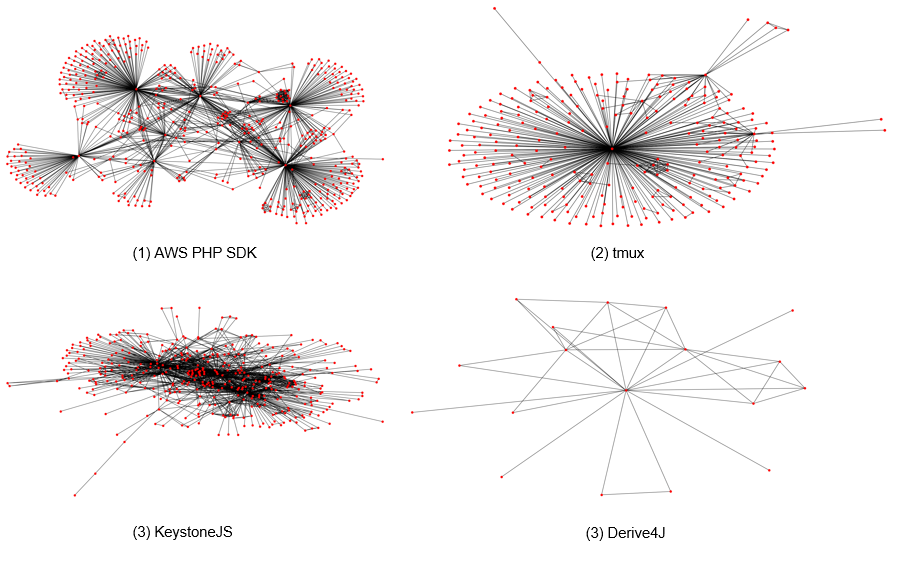
\includegraphics[width=.95\textwidth]{network_plots.PNG}
\caption{Example networks from the data set.}
\label{network_plots}
\end{figure*}

Table \ref{network_summary} shows the summary statistics for each of the network structure variables. For the Gini coefficient, the summary statistics show a tight cluster of stakeholder networks with a moderate level of concentration, contrasted with a smaller number of highly- and lowly-concentrated networks on either end of the distribution. The statistics for average minimum path indicate that most of the stakeholder networks are, per Watts and Strogatz \cite{watts}, relatively small-worlds, although the data set does show substantial variability in the breadth of the networks. The clustering coefficient takes on the most diverse distribution of values, ranging from networks with virtually no localized clustering, such as the network for tmux in Figure \ref{network_structure}, to highly integrated networks, such as the network for KeystoneJS.

\begin{table}
\caption{Summary Statistics for Network Variables}
\label{network_summary}
\begin{tabular}{llllll}
\hline\noalign{\smallskip}
Variable & Min & 25\% & Median & 75\% & Max  \\
\noalign{\smallskip}\hline\noalign{\smallskip}
Gini Coeff. & 0.29 & 0.54 & 0.57 & 0.59 & 0.70 \\
Avg. Min. Path & 1.40 & 2.01 & 2.15 & 2.33 & 3.05 \\
Clustering Coeff. & 0.00 & 0.52 & 0.63 & 0.70 & 0.88 \\
\noalign{\smallskip}\hline
\end{tabular}
\end{table}

The scatter plots in Figure \ref{network_structure_scatter} show that crowd-sourcing occurs at varying intensities across all network types. The wide distribution of crowd-sourcing intensities across network structures also makes statistical inference more reliable. Specifically, the distribution allows the models to capture how crowd-sourcing interacts with network structure without having to worry about (a) combinations of crowd-sourcing and network structure that fall outside the range of observed values in the data set and (b) excessive collinearity between the covariates. This property makes the data set ideal for assessing how network structure impacts the effectiveness of crowd-based requirements processes.

\begin{figure*}
  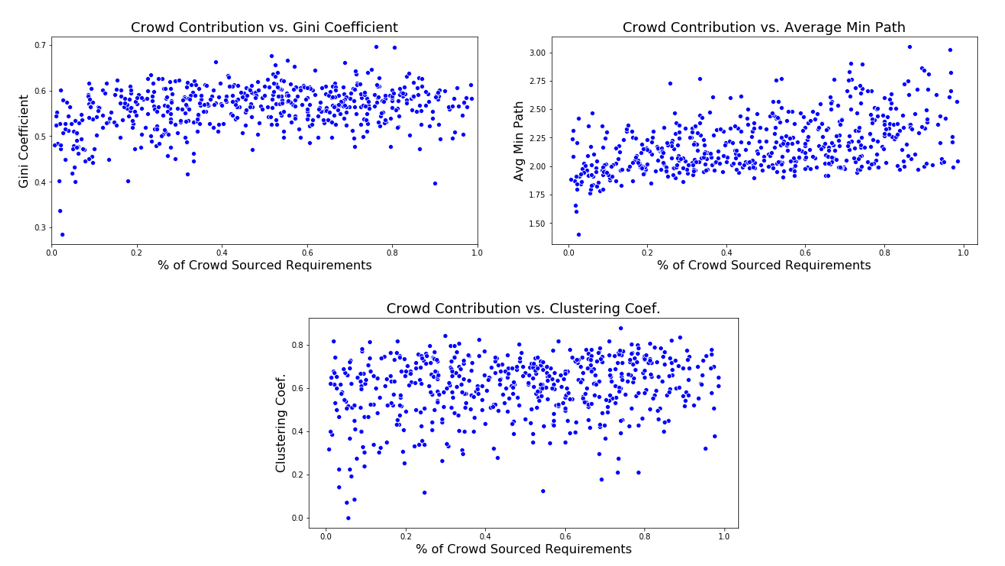
\includegraphics[width=.95\textwidth]{network_structure_scatter.PNG}
\caption{Scatter plots from the input data set.}
\label{network_structure_scatter}
\end{figure*}

\subsection{Regression Results}

\subsubsection{Close-Out Time}

Within the data set, the average number of days a requirement remains active ranges from less than a day to several years. On average, most projects closeout requirements within three months, although the data set does included several projects with very long average close-out times. The results of the KS test fail to reject the null hypothesis that close-out time follows a Gamma distribution, making the Gamma GLM a reasonable model choice.

\begin{figure*}
  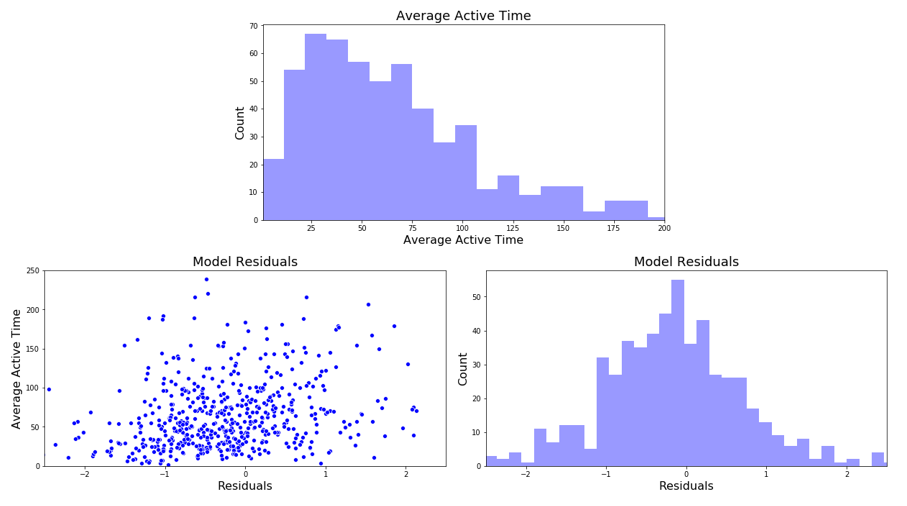
\includegraphics[width=.95\textwidth]{active_time_results.PNG}
\caption{Average requirement close-out time distribution and regression results.}
\label{active_time_results}
\end{figure*}

Table \ref{active_time_regression} shows the regression results. All seven variables are statistically significant at the one percent significance level. The residual plot in Figure \ref{active_time_results} shows no relationship between requirement close-out time and the residuals, which means the results do not raise any concerns about biased estimators.

\begin{table}
\caption{Regression on Requirement Active Time}
\label{active_time_regression}
\begin{tabular}{lll}
Gamma GLM | Pseudo $R^2$: 0.51 \\
\hline\noalign{\smallskip}
Variable & Coefficient & p-value  \\
\noalign{\smallskip}\hline\noalign{\smallskip}
Intercept & 0.98 & 0.05 \\
Crowd Percentage & 4.36 & $\leq 0.01$  \\
Avg Min Path & 0.75 & $\leq 0.01$ \\
Clustering x Crowd Percentage & 3.06 & $\leq 0.01$ \\
Avg Min Path x Crowd Percentage & -1.29 & $\leq 0.01$ \\
Gini Coefficient x Crowd Percentage & -4.75 & $\leq 0.01$ \\
Project Age & 0.0005 & $\leq 0.01$ \\
Nodes & 0.0004 & $\leq 0.01$ \\
\noalign{\smallskip}\hline
\end{tabular}
\end{table}

Figure \ref{active_time_marginal} shows how the marginal effect of crowd percentage changes with network structure. For dispersed networks with high concentration and low levels of localized clustering, increasing crowd participation does not result in substantial increases in requirement close-out time. Networks with the opposite characteristics suffer accelerating requirement close-out times as crowd percentage increases, which indicates that project teams cannot keep up with a growing backlog of crowd-sourced requirements. These results point to stakeholder network with well-defined hubs as a more effective configuration.

\begin{figure*}
  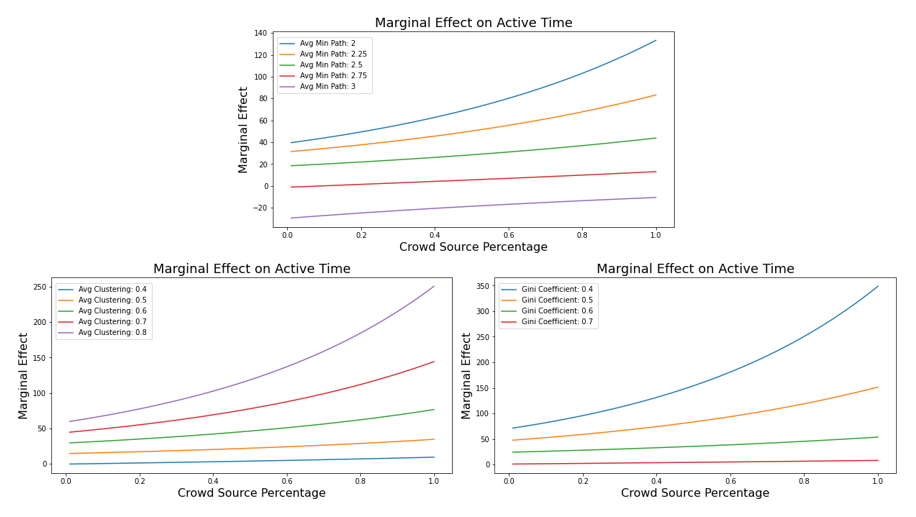
\includegraphics[width=0.95\textwidth]{active_time_marginal.PNG}
\caption{Marginal effects on requirement close-out time as a function of crowd-sourcing.}
\label{active_time_marginal}
\end{figure*}

\subsubsection{Response Time}

The average response times in the data set range from within a day to slightly over a year. As the histogram in Figure \ref{reaction_time_results} shows, the observations follow a lifetime distribution with a long right tail. On average, most projects teams respond to requirements within a month.

\begin{figure*}
  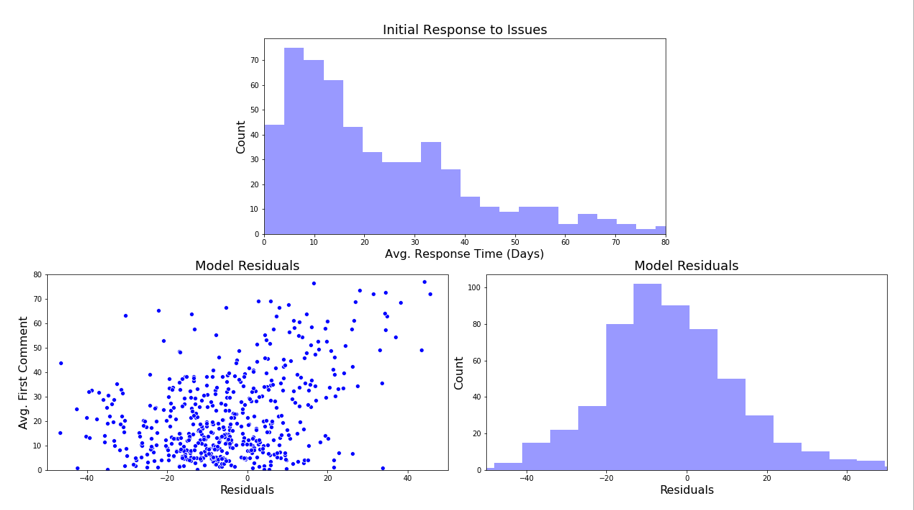
\includegraphics[width=0.95\textwidth]{reaction_time_results.PNG}
\caption{Average requirement response time distribution and regression results}
\label{reaction_time_results}
\end{figure*}

Table \ref{reaction_time_regression} shows the regression results for requirement response time. For response time, the OLS model had an adjusted $R^2$ of 0.56 compared to a pseudo-$R^2$ of 0.43 for the Gamma GLM. Due to better model performance and because the model appeared to conform to the Gauss-Markov assumptions, the research team opted to use the OLS model. The OLS model includes eight variables, all of which demonstrate statistical significance at the ten percent significance level. As shown in Figure \ref{reaction_time_results}, the residuals approximate a normal distribution and do not correlate with the response variable. Therefore, the model adheres to the Gauss-Markov assumptions and does not appear likely to suffer from biased estimators.

\begin{table}
\caption{Regression on Reaction Time}
\label{reaction_time_regression}
\begin{tabular}{lll}
OLS Regression | $R^2$: 0.57 | Adjusted $R^2$: 0.56 \\
\hline\noalign{\smallskip}
Variable & Coefficient & p-value  \\
\noalign{\smallskip}\hline\noalign{\smallskip}
Crowd Percentage Sq. & 69.97 & 0.01 \\
Gini Coefficient & 152.50 & 0.03 \\
Gini X Crowd Pct & -274.34 & $\leq 0.01$ \\
Avg Clustering & -50.57 & $\leq 0.01$ \\
Avg Clustering x Crowd Pct & 34.38 & $\leq 0.01$ \\
Avg Min Path & 34.72 & $\leq 0.01$ \\
Project Age & 0.02 & $\leq 0.01$ \\
Topic 2 & -69.40 & 0.07 \\
\noalign{\smallskip}\hline
\end{tabular}
\end{table}

The marginal effect plots in Figure \ref{reaction_time_marginal} demonstrate that the impact of crowd-sourcing changes dramatically with the structure of the networks. Whereas increasing crowd-sourcing reduces reaction time for networks with high concentration and low localized clustering, the opposite holds for networks with high localized clustering and low concentration. Networks with faster response times have a hub-and-spoke structure, compared with a more dispersed, web-like structure for lower performing networks. These results suggest that project teams perform well when they have delineated areas of responsibility, which allows them to concentrate on and respond to a smaller number of requirements from the crowd. Moreover, the results show that the marginal impact on response time increases with the level of crowd-sourcing in the system, which implies that crowd-sourcing faces decreasing marginal returns.

\begin{figure*}
  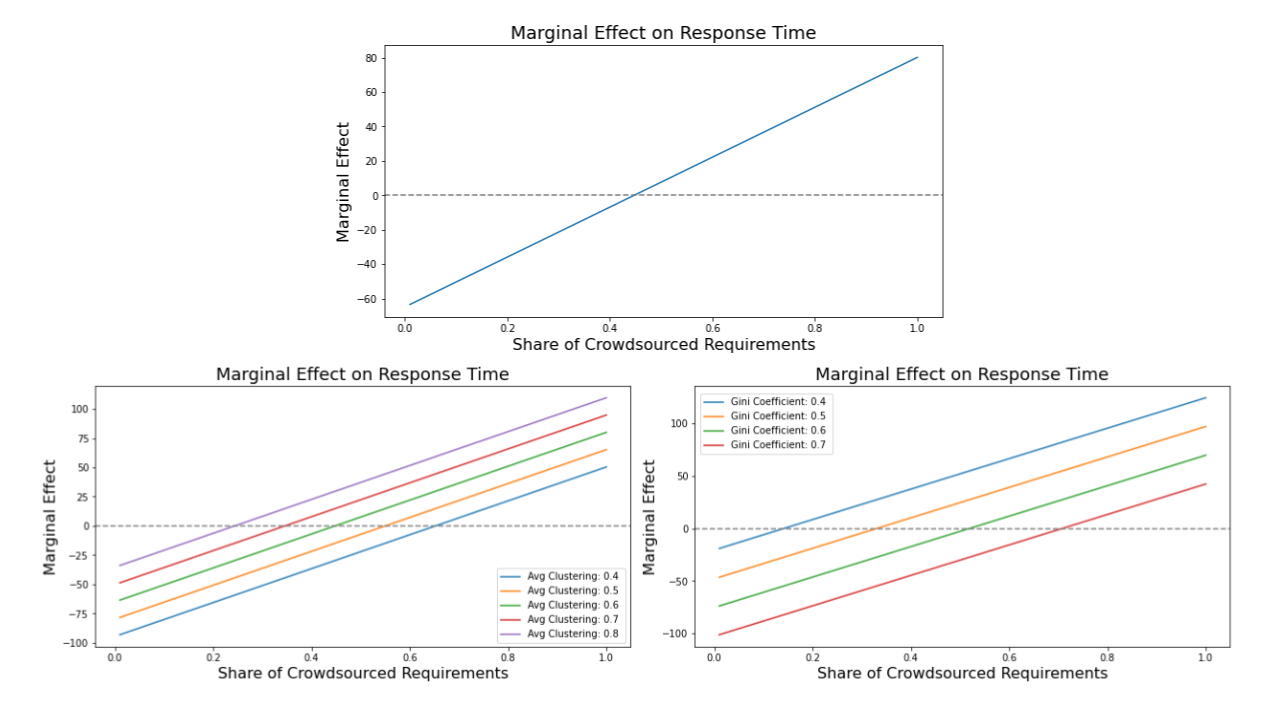
\includegraphics[width=0.95\textwidth]{reaction_time_marginal.PNG}
\caption{Marginal effects on reaction time as a function of crowd-sourcing.}
\label{reaction_time_marginal}
\end{figure*}

\subsubsection{Comment Activity}
\label{comment_activity}

As noted in Section \ref{measures_of_effectiveness}, average comment activity indicates stronger engagement in the requirements formation process \cite{toral}. Therefore, higher average comment activity represents a positive outcome. Figure \ref{comment_activity_results} includes a histogram showing the distribution of average comments within the data set. The histogram shows that average comment activity has an approximately normal distribution and ranges from 1-8 comments per requirement. While the histogram for comment activity appears normal, since it has a positive domain, modeling comment activity with a Gamma distribution remains a reasonable choice. Since the Gamma distribution constitutes a sum of Exponential random variables, the Central Limit Theorem implies that a Gamma distribution can approximate a normal distribution if parameterized properly \cite{wackerly}. Indeed, the results of the KS tests show that the comment activity data fit both the normal and Gamma distributions well under their maximum likelihood estimates. Under these conditions, either a Gamma GLM or an OLS model are sensible options. In this case, the research team favored the Gamma GLM due to materially better model performance.

\begin{figure*}
  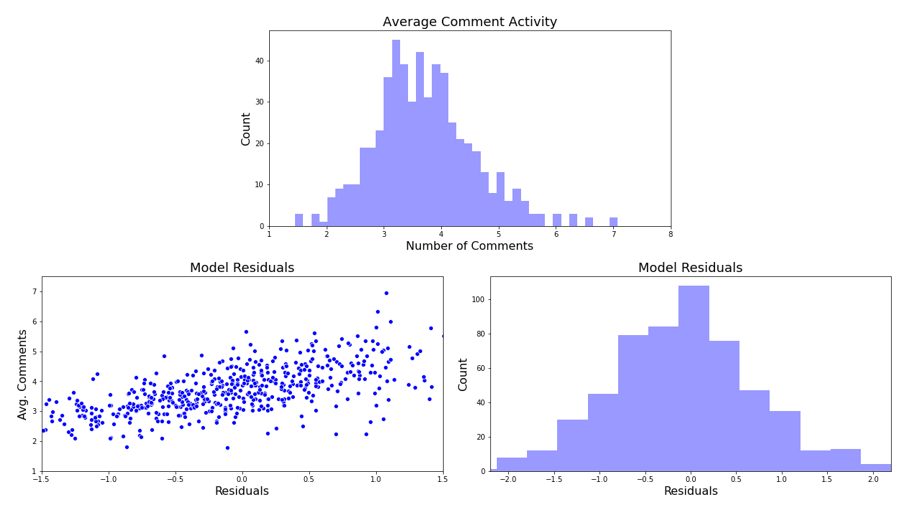
\includegraphics[width=0.95\textwidth]{comment_activity_results.PNG}
\caption{Comment activity distribution and regression results.}
\label{comment_activity_results}
\end{figure*}

Table \ref{comment_activity_regression} presents the regression results. The model contains 21 variables, including several of the topic content variables introduced in Section \ref{topic_modeling}. Each variable in the regression model is statistically significant at the five percent significance level. Residual plots for the regression appear in Table \ref{comment_activity_results}. The residual plots show a positive correlation between the residuals and the response variables. However, a linear regression between the dependent variables and the residuals reveals no statistically significant relationship, leading to no concern about biased estimators for this model.

\begin{table}
\caption{Regression on Comment Activity}
\label{comment_activity_regression}
\begin{tabular}{lll}
Gamma GLM | Pseudo $R^2$: 0.50 \\
\hline\noalign{\smallskip}
Variable & Coefficient & p-value  \\
\noalign{\smallskip}\hline\noalign{\smallskip}
Intercept & 0.74 & $\leq 0.01$ \\
Crowd Percentage & 4.47 & $\leq 0.01$ \\
Crowd Percentage Sq. & -3.10 & $\leq 0.01$ \\
Crowd Percentage Cu. & 1.69 & $\leq 0.01$ \\
Avg Min Path Sq. & 0.40 & $\leq 0.01$ \\
Avg Min Path x Crowd Pct & -2.72 & $\leq 0.01$ \\
Gini Coefficient Sq & 2.85 & 0.03 \\
Gini. x Avg Min Path & -2.52 & $\leq 0.01$ \\
Gini. x Clustering & 2.04 & $\leq 0.01$ \\
Gini. x Avg Min Path x Crowd Pct & 3.33 & $\leq 0.01$ \\
Gini. x Clustering x Crowd Pct & -12.46 & $\leq 0.01$ \\
Avg Clustering Sq. & 1.53 & $\leq 0.01$ \\
Clustering x Avg Min Path & -1.82 & $\leq 0.01$ \\
Clustering x Avg Min Path x Crowd Pct & 2.43 & $\leq 0.01$ \\
Avg First Comment & -0.002 & $\leq 0.01$ \\
Avg Active Time & 0.001 & $\leq 0.01$ \\
Topic 2 & 1.00 & $\leq 0.01$ \\
Topic 5 & 0.37 & $\leq 0.01$ \\
Topic 13 & -0.38 & 0.03 \\
Topic 18 & -0.82 & $\leq 0.01$ \\
Topic 2 x Topic 18 & 4.41 & $\leq 0.01$ \\
\noalign{\smallskip}\hline
\end{tabular}
\end{table}

The intensity of crowd-sourcing and the structure of the stakeholder network have a greater effect on comment activity than on any other measure of effectiveness. The overall trend shows an increase in comment activity for systems with very low and very high levels of crowd-sourcing. Positive marginal effects at lower levels of crowd-sourcing almost certainly reflects better feedback from the crowd. The reduced effect on comment activity at moderate levels of crowd-sourcing may suggest that the project team engages less on individual issues as they spend more time implementing a higher volume of requirements from the crowd. At high levels of crowd-sourcing, the increase in comment activity from crowd members could outweigh lower comment activity from the project team, leading marginal effect to increase once more. This explanation, of course, remains speculative and subject to further investigation.

Generally, less locally clustered and less concentrated networks generate more comment activity, although the difference for network concentration diminishes at higher levels of crowd-sourcing. For dispersed networks, the marginal effect on comment activity remains relatively flat at all levels of crowd-sourcing, while networks with a lower average minimum path experience a more pronounced decrease at moderate ranges. Since network with less localized clustering perform better with respect to comment activity and concentration has a limited effect, these results remain consistent with the hypothesis that stakeholder networks with multiple hubs contend with increases in crowd participation most effectively.

\begin{figure*}
  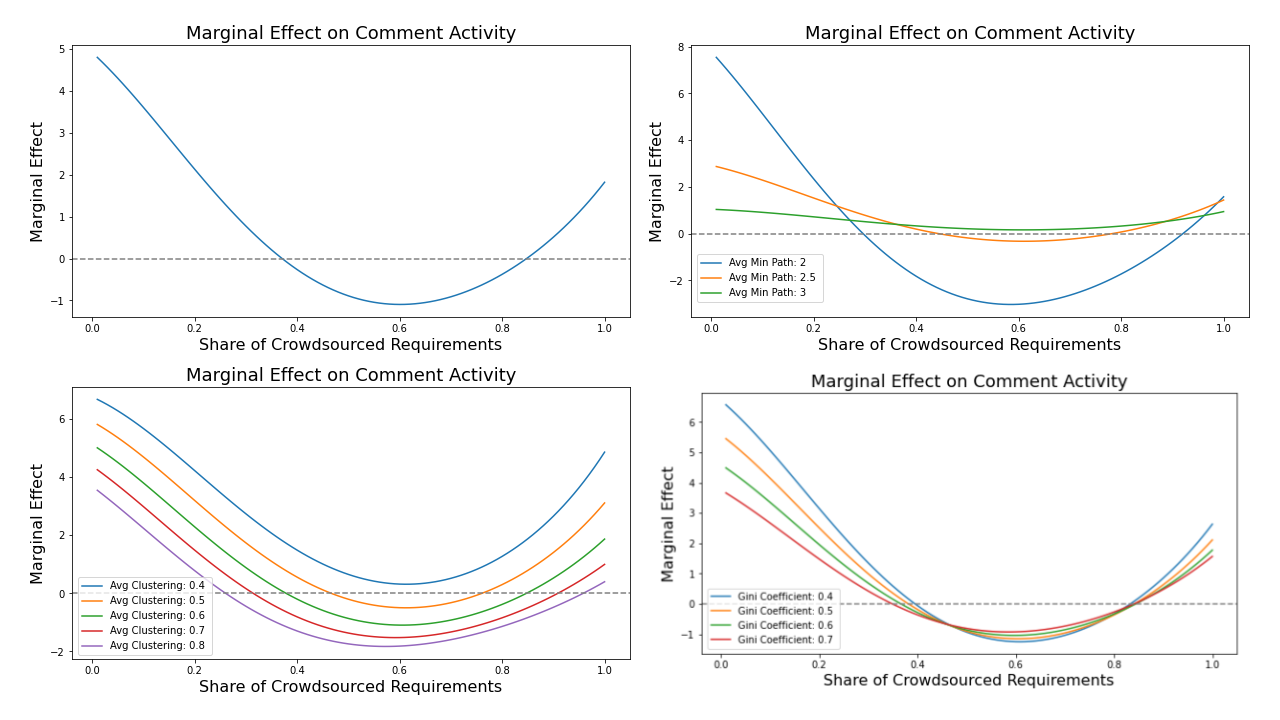
\includegraphics[width=0.95\textwidth]{comment_activity_marginal.PNG}
\caption{Marginal effects on comment activity as a function of crowd-sourcing.}
\label{comment_activity_marginal}
\end{figure*}

\subsubsection{Issues Per Crowd Member}

The average number of issues per crowd member measures the intensity of engagement between the project team and the crowd. Repeat issue submissions show that a crowd member has remained engaged with the project over time. As shown in Figure \ref{issues_per_user_results}, for most projects, each crowd member submits relatively few requirements. However, the distribution has a long right tail, and some projects average several dozen issues per crowd member. The results of the KS test validate that the variable conforms to a Gamma distribution, per the assumptions of the Gamma GLM.

\begin{figure*}
  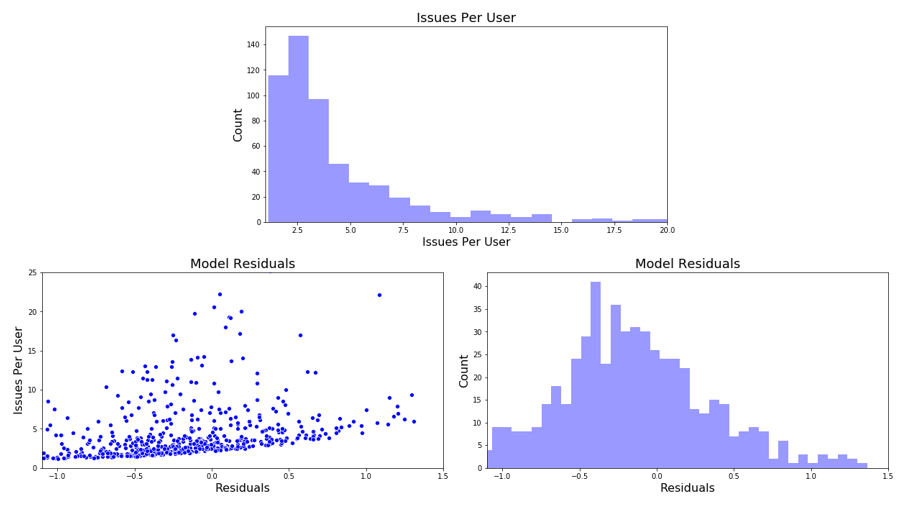
\includegraphics[width=0.95\textwidth]{issues_per_user_results.PNG}
\caption{Distribution of issues per user and regression results.}
\label{issues_per_user_results}
\end{figure*}

The regression results for the network and crowd-sourcing variables appear in Table \ref{issues_per_user_regression}. In contrast to the other regressions, the variable selection process only selected a small number of variables for this regression. The model includes three variables, each of which reveals statistical significance at the one percent significance level. Of the network structure variables, only average minimum path appears in the equation. Its effect, however, does not change with the level of crowd sourcing. Other network structure variables do not have a statistically significant effect when included in the regression.  This leads to the conclusion that, while the level of crowd-sourcing affects the number of issues per crowd member, the structure of the stakeholder network does not. 

Figure \ref{issues_per_user_results} shows a positive correlation between issues per crowd member and the residuals. A linear regression of the residuals against the dependent variables shows a slight positive correlation between crowd percentage and the residuals, and a slight negative correlation between crowd percentage squared and the residuals. These results imply bias toward zero for both of the coefficients, meaning the model probably overestimates the effect of crowd-sourcing. However, the base and squared crowd percentage term both have roughly the same coefficient in the residual regression, meaning the positive-to-negative cross-over point remains unbiased, even though the GLM overestimates the overall effect of crowd-sourcing.

\begin{table}
\caption{Regression on Issues Per User}
\label{issues_per_user_regression}
\begin{tabular}{lll}
Gamma GLM | Pseudo $R^2$: 0.64 \\
\hline\noalign{\smallskip}
Variable & Coefficient & p-value  \\
\noalign{\smallskip}\hline\noalign{\smallskip}
Intercept & 2.17 & $\leq 0.01$ \\
Crowd Percentage & -7.90 & $\leq 0.01$ \\
Crowd Percentage Squared & 6.40 & $\leq 0.01$  \\
Avg Min Path & 0.52 & $\leq 0.01$  \\
\noalign{\smallskip}\hline
\end{tabular}
\end{table}

The coefficients indicate that additional crowd-sourcing decreases the number of issues per contributor for projects that source less that 65\% of their requirements from the crowd, and increases the number of issues per user beyond that threshold. These results imply uneven contributions from the crowd---for projects that crowd-source a high proportion of their requirements, a small group of highly active crowd members generate most of the requirements. The structure of the stakeholder network, however, does not appear to have any effect.

\subsubsection{Issue Volume}

Issue volume measures the number of new requirements per quarter. The histogram in Figure \ref{issue_volume_results} shows that the distribution of issue volume in the data set follows a lifetime distribution with a long right tail, with a maximum value of 84 new requirements per quarter. KS test results show that issue volume follows a Gamma distribution, justifying the choice to employ a Gamma GLM model. As discussed above, while crowd based requirements engineering generally seeks to increase the volume of requirements, too many incoming requirements can overwhelm the project team. Therefore, a complete analysis of this variable must include an assessment of the trade-off between issue volume and other measures of effectiveness.

\begin{figure*}
  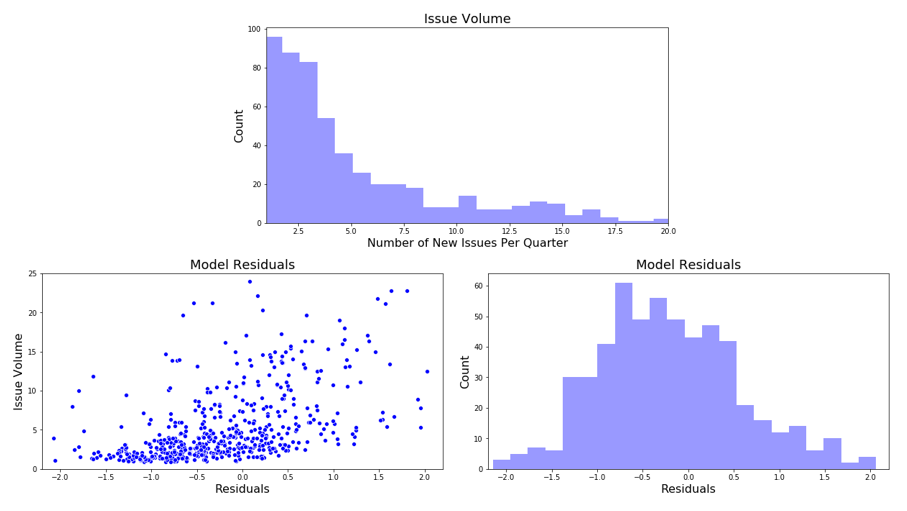
\includegraphics[width=0.95\textwidth]{issue_volume_results.PNG}
\caption{Issue volume distribution and regression results.}
\label{issue_volume_results}
\end{figure*}

The regression results for the GLM appear in Table \ref{issue_volume_regression}. Each of the seven variables in the model are statistically significant at the ten percent significance level. Due to the small magnitude of the coefficient, the average minimum path interaction term is not practically significant. The interaction terms suggest that the impact of crowd-sourcing does not change with the level of concentration in the network, although it does change with the level of localized clustering in the network. The residual plot in Figure \ref{issue_volume_results} shows slight positive correlation between the residuals and issue volume. However, a linear regression of the residuals against the dependent variable does not show any correlation, which means the regression does not have biased estimators.

\begin{table}
\caption{Regression on Issue Volume}
\label{issue_volume_regression}
\begin{tabular}{lll}
Gamma GLM | Pseudo $R^2$: 0.66 \\
\hline\noalign{\smallskip}
Variable & Coefficient & p-value  \\
\noalign{\smallskip}\hline\noalign{\smallskip}
Intercept & 1.87 & $\leq 0.01$ \\
Crowd Percentage & -4.09 & $\leq 0.01$  \\
Crowd Percentage Squared & 3.42 & $\leq 0.01$  \\
Clustering & -1.42 & $\leq 0.01$  \\
Gini Coefficient & 3.49 & $\leq 0.01$  \\
Clustering x Crowd Percentage & 2.15 & $\leq 0.01$  \\
Avg Min Path x Crowd Percentage & -0.44 & 0.06 \\
Total Contributors & 0.05 & $\leq 0.01$ \\
\noalign{\smallskip}\hline
\end{tabular}
\end{table}

These results mirror the observations in Section \ref{comment_activity}. In particular, they show that additional crowd-sourcing reduces issue volume for projects with less crowd-sourcing, but increases issue volume for projects with more crowd-sourcing. Additionally, Figure \ref{issue_volume_marginal} shows that the biggest marginal increase in issue volume occurs in projects with a high level of localized clustering. 

\begin{figure*}
  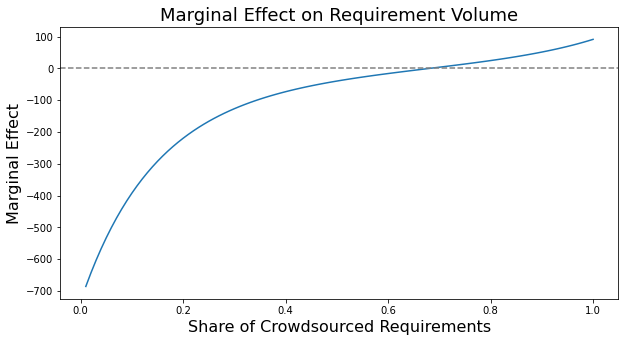
\includegraphics[width=0.95\textwidth]{issue_volume_marginal.PNG}
\caption{Marginal effects on issue volume as a function of crowd-sourcing.}
\label{issue_volume_marginal}
\end{figure*}

As noted in Section \ref{measures_of_effectiveness}, an increase in issue volume can represent a positive or a negative outcome, depending on the circumstances. Systems engineers can determine the costs and benefits of an increase in issue volume by plotting the trade-off space between issue volume and other measures of effectiveness. Figure \ref{leaflet_trade_space} shows the trade-off analysis for LeafletJS, a JavaScript geospatial library. In this example, an increase in issue volume results in longer response and close-out times and less comment activity on each requirement, reflecting a trade-off between levels of crowd engagement and the comprehensiveness of the requirement set. Projects will face different trade-offs depending on the structure of their stakeholder network and the current level of crowd-sourcing. Trade-off plots provide systems engineers with the ability to make an informed decision based on the specific circumstances of their project.

\begin{figure*}
  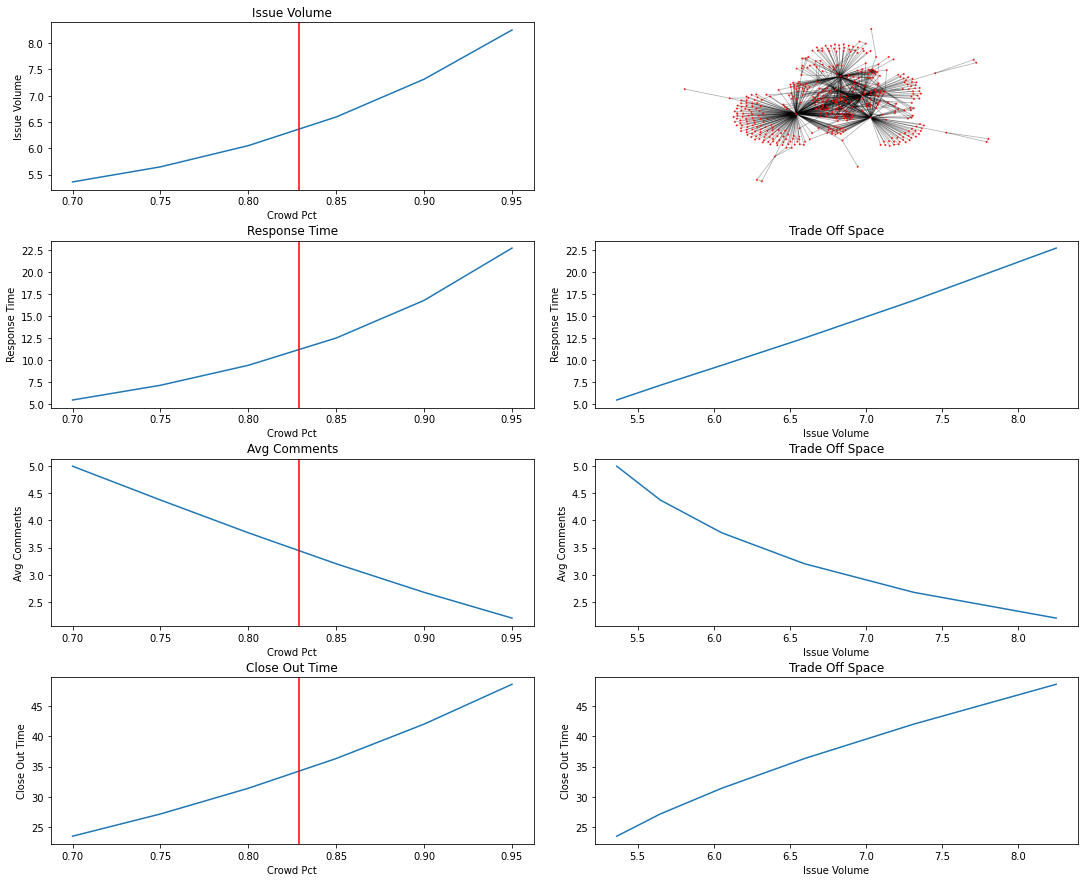
\includegraphics[width=0.95\textwidth]{leaflet_trade_space.png}
\caption{Trade-off space as issue volume increase for LeafletJS.}
\label{leaflet_trade_space}
\end{figure*}

\section{Conclusion}

\subsection{Discussion}

From a practical perspective, the results in Section \ref{results_section} help systems engineers address the following question: Given the current structure of the stakeholder network for my project, should I encourage more crowd participation? Answering that questions requires systems engineers to make a conscious trade-off between various measures of effectiveness.

Under all circumstances, increasing crowd participation increases the amount of time it takes to closeout requirements. However, networks with low concentration suffer a particularly dramatic increase, as do narrow and locally clustered networks. While crowd-sourcing always lengthens close-out time, increasing crowd participation improves contributor response time to new requirements for highly concentrated networks with low localized clustering. By contrast, more crowd-sourcing results in slower response times for low concentration stakeholder networks with high localized clustering. For these measures of effectiveness, stakeholder networks with multiple concentrated hubs perform best.

For issue volume the marginal effect of crowd-sourcing changes as the level of crowd-sourcing increases. Additional crowd-sourcing results in lower issue volume for projects with low crowd participation, but higher issue volume for projects with high crowd participation. The cross-over point occurs at a crowd-sourcing rate of 55-60\%. For systems with crowd-sourcing rates of 35-80\%, which roughly covers the interquartile range of the data set, network structure has minimal impact on the marginal effect of crowd-sourcing, although noticeable differentiation occurs based on localized clustering at the extremes of the distribution. Again, the outcomes favor stakeholder networks with disjoint hubs.

More crowd-sourcing has a positive effect on comment activity for systems with low and high levels of crowd-sourcing. The marginal effect decreases and in some cases becomes negative for projects that crowd-sourcing a moderate share of requirements. Less locally clustered stakeholder networks perform best across the full range of crowd-sourcing intensities. Highly concentrated networks have a slightly lower, but still positive effect on comment activity at lower levels of crowd-sourcing, but the difference disappears at moderate and high levels of crowd-sourcing. These patterns suggest that, at moderate levels of crowd-sourcing, members of the project team spend less time engaging with the crowd and more time on implementation. As crowd-sourcing increases further, increased comment volume from the crowd counterbalances this effect. The stronger performance of networks with less localized clustering combined with the minimal effect of network concentration at high levels of crowd-sourcing lends support to the hypothesis that hub-and-spoke networks handle crowd-based requirements processes most effectively.

Overall, the results suggest that stakeholder networks with multiple, relatively disjoint hubs have the best risk-reward trade-off when employing crowd-based requirements processes. Referencing Figure \ref{network_plots}, the most effective stakeholder networks look similar to the AWS project in the top left. These results support Toral, Martinez-Torres, and Barrero's \cite{toral} conclusions, which suggest that more concentrated network structures produce better project management outcomes. The presence of disjoint hubs suggests that the most efficient projects have several contributors, each of whom specialize in a particular aspect of the codebase. Taking advantage of this kind of network structure requires systems engineers to design processes for assigning each incoming requirement to the proper contributor. For example, Dalpiaz, Ferrari, Franch, and Palomares propose a process that uses natural language processing to triage and assign requirements \cite{dalpiaz}.

Moreover, encouraging additional crowd-sourcing makes the most sense for projects that currently engage in a low-to-moderate degree of crowd-sourcing, or those that crowd-source less than 65\% of their requirements from the crowd. The data shows that, for any network structure, sourcing too many requirements from the crowd results in a growing backlog and low engagement, validating the concerns that Snijders and high colleagues have raised \cite{snijders}. 

\subsection{Limitations}
\label{limitations}

Readers should keep in mind several limitations of this study. First, although the scope of the research covers many of the proposed benefits and drawbacks mentioned in the crowd-based requirements engineering literature, it does not include all of them. Lim and his colleagues, for instance, speculate that crowd-based requirements engineering results in higher quality requirements \cite{stakerare} and helps systems engineers understand unanticipated use cases more quickly. Average comment activity captures the level of engagement on requirements, but does not directly measure their quality. Likewise, the data set does not measure how crowd-sourcing affects how the project team understands the use cases for a system or capture the level of enthusiasm for a product amongst the user base. Groen and his colleagues \cite{groen} cite increased enthusiasm as a potential benefit of crowd-sourcing. Finally, the analysis does not consider the impact of crowd-sourcing on the prioritization of individual requirements. Lim, et al. raise the concern that crowd-based requirements processes might result in a tendency for project teams to prioritize requirements from the most active stakeholders \cite{stakenet}. 

Additionally, the data set only contains open-source software projects, which limits how well the results generalize. On average, since they come from the software development community, users of open-source software have an unusually keen understanding of a package's technical details. As such, they may engage with the requirements process more actively and effectively than users of a consumer-facing software product. Expanding from software to physical products would present even more challenges due to, in most cases, longer feedback cycles and less mutable specifications. Moreover, while the data set covers a broad range of open-source projects, it only includes widely adopted packages with at least thirty requirements. The results may not apply equally well to smaller open-source packages with less active user bases.

\subsection{Future Research}

This research prompts several questions that could serve as the basis for follow-on analysis. First, measures of effectiveness in this study assume that lack of attention from the project team leads to less engaged crowd members over time. Future research could evaluate this claim empirically by examining the relationship between response times from the project team and the probability that a crowd member submits more requirements in the future.

Second, the results in this paper indicate that stakeholder networks with multiple, disjoint hubs absorb additional crowd participation most effectively. A reasonable hypothesis to explain this phenomenon is that each hub is a contributor with a particular area of specialization. These stakeholder networks may perform better as crowd-sourcing expands because each contributor only needs to focus on a small subset of incoming requirements. An investigation to determine whether different hubs in these networks indeed specialize based on requirement type could yield valuable insights.

Third, one of the proposed benefits of crowd-based requirements engineering is that it leads to the generation of new requirements that systems engineers would not have identified if they had not engaged with the crowd. If crowd members and project team members produce similar requirements, that would negate this benefit. A research effort to determine the degree to which crowd-generated requirements differ from internally sourced requirements could help shed light on this issue.

Fourth, as suggested in Section \ref{trade-off}, future research could develop more sophisticated models to analyze the trade-off space between various measures of effectiveness. These models should account for the change in network structure that occurs when systems source additional requirements from the crowd, and include sensitivity analysis that quantifies how a change in network structure would impact the trade-off space.

Finally, this study considers stakeholder networks as a snapshot in time. In reality, the structure of these networks evolves along with their their performance characteristics. An effort to study how these stakeholder networks arrived at their current structure could help systems engineers design interventions that will guide their interactions with the crowd toward a positive outcome.

\subsection{Summary}

This study used a GitHub data set consisting of project management artifacts from a curated set of 562 open-source software projects to evaluate the impact of stakeholder network structure on the effectiveness of crowd-based requirements processes. For four out of five measures of effectiveness, statistical analysis shows that the marginal impact of additional crowd-sourcing changes with the structure of the stakeholder network and the current level of crowd-sourcing for the project. The results suggest that open-source software projects whose stakeholder networks have multiple, disjoint hubs and a low level of localized clustering absorb additional crowd engagement most effectively and imply that systems engineers should encourage contributors to specialize in distinct aspects of the code base and establish processes to route incoming requirements to the proper contributor. Moreover, the analysis indicates that additional crowd-sourcing is most beneficial for projects that currently have a low-to-moderate degree of crowd engagement, or those that presently crowd-source fewer than 65\% of requirements. Increasing crowd participation beyond that point leads to diminishing marginal returns. While this research establishes a connection between stakeholder network structure and the effectiveness of crowd-sourcing within the context of open-source software, determining the degree to which the results generalize to other systems requires further investigation.

 \section*{Conflict of interest}

The authors declare that they have no conflict of interest.

\section*{Availability of data and material}

Data is available at https://github.com/MthwRobinson/sh-network-paper/blob/master/github\_data.csv.

\section*{Code availability}

Code is available at https://github.com/MthwRobinson/sh-network-paper.

\section*{Author contributions}

The material in this paper has been abstracted and developed from a dissertation submitted to the  George Washington University in partial fulfillment of the requirements for Matthew Robinson's Ph.D. degree.

\begin{thebibliography}{}

\bibitem{aizawa}
Aizawa, A (2003) An information-theoretic perspective of tf–idf measures. Information Processing \& Management, 39(1): 45-65.

\bibitem{anscombe}
Anscombe, FJ, \& Tukey, JW (1963) The examination and analysis of residuals. Technometrics, 5(2): 141-160.

\bibitem{blei}
Blei, DM, Ng, AY, \& Jordan, MI (2003) Latent dirichlet allocation. Journal of machine Learning research, 3(Jan): 993-1022.

\bibitem{javascript}
Chen, C. Awesome JavaScript, GitHub Repository, https://github.com/sorrycc/awesome-javascript (2019)

\bibitem{python}
Chen, V (2019) Awesome Python GitHub Repository. https://github.com/vinta/awesome-python Accessed 15 June 2019

\bibitem{dalpiaz}
Dalpiaz, F, Ferrari, A, Franch, X, \& Palomares, C (2018) Natural language processing for requirements engineering: The best is yet to come. IEEE software, 35(5): 115-119.

\bibitem{damian}
Damian, D, Marczak, S, \& Kwan, I (2007) Collaboration patterns and the impact of distance on awareness in requirements-centred social networks. In 15th IEEE International Requirements Engineering Conference (RE 2007): 59-68.

\bibitem{derkson}
Derksen, S, \& Keselman, HJ (1992) Backward, forward and stepwise automated subset selection algorithms: Frequency of obtaining authentic and noise variables. British Journal of Mathematical and Statistical Psychology, 45(2): 265-282.

\bibitem{fahrmeir}
Fahrmeir, L, Kneib, T, Lang, S, \& Marx, B (2007) Regression. Springer-Verlag Berlin, Heidelberg: 300-301.

\bibitem{cpp}
Fallahi, F, (2019) Awesome C++ GitHub Repository. https://github.com/fffaraz/awesome-cpp Accessed 15 June 2019

\bibitem{finkelstein}
Finkelstein, A (1994) Requirements Engineering: a review and research agenda. In Proceedings of 1st Asia-Pacific Software Engineering Conference: 10-19.

\bibitem{ferrari}
Ferrari, S, \& Cribari-Neto, F (2004) Beta regression for modelling rates and proportions. Journal of applied statistics, 31(7): 799-815.

\bibitem{friedman}
Friedman, J, Hastie, T, \& Tibshirani, R (2001) The elements of statistical learning (Vol. 1, No. 10). Springer series in statistics, New York: 60-61.

\bibitem{gerth}
Gerth, RJ, Burnap, A, \& Papalambros, P (2012) Crowdsourcing: A primer and its implications for systems engineering. Michigan University, Ann Arbor.

\bibitem{gini}
Gini, C (1912) Variabilità e mutabilità. Reprinted in Memorie di metodologica statistica (Ed. Pizetti E, Salvemini, T). Libreria Eredi Virgilio Veschi, Rome.

\bibitem{gini2}
Gini, C (1921) Measurement of inequality of incomes. The Economic Journal, 31(121): 124-126.

\bibitem{groen}
Groen, EC, Seyff, N, Ali, R, Dalpiaz, F, Doerr, J, Guzman, E, ... \& Stade, M (2017) The crowd in requirements engineering: The landscape and challenges. IEEE software, 34(2): 44-52.

\bibitem{holland}
Holland, PW, \& Leinhardt, S (1971) Transitivity in structural models of small groups. Comparative group studies, 2(2): 107-124.

\bibitem{howe2}
Howe, J (2008) Crowdsourcing: How the power of the crowd is driving the future of business. Random House.

\bibitem{howe}
Howe, J (2006) The rise of crowd-sourcing, Wired magazine 14, no. 6: 1-4.

\bibitem{hosseini}
Hosseini, M, Phalp, KT, Taylor, J, \& Ali, R (2014) Towards crowdsourcing for requirements engineering.

\bibitem{iyer}
Iyer, DG, \& Lyytinen, K (2019) Requirements engineering (RE) effectiveness in open source software: the role of social network configurations and requirements properties. Requirements Engineering, 5, 15-2019.

\bibitem{java}
Kull, A (2019) Awesome Java GitHub Repository. https://github.com/akullpp/awesome-java Accessed 15 June 2019.

\bibitem{latoza}
LaToza, TD, \& Van Der Hoek, A (2015) Crowdsourcing in software engineering: Models, motivations, and challenges. IEEE software, 33(1): 74-80.

\bibitem{levy}
Levy, M., Hadar, I., \& Te'eni, D.,. A gradual approach to crowd-based requirements engineering: The case of conference online social networks, 2015 IEEE 1st International Workshop on Crowd-Based Requirements Engineering (CrowdRE), 25-30, IEEE (2015)

\bibitem{stakerare}
Lim, SL, \& Finkelstein, A (2011) StakeRare: using social networks and collaborative filtering for large-scale requirements elicitation. IEEE transactions on software engineering, 38(3): 707-735.

\bibitem{stakenet}
Lim, SL, Quercia, D, \& Finkelstein, A (2010) StakeNet: using social networks to analyse the stakeholders of large-scale software projects. In 2010 ACM/IEEE 32nd International Conference on Software Engineering, Vol. 1: 295-304.

\bibitem{lim}
Lim, SL, \& Ncube, C (2013) Social networks and crowdsourcing for stakeholder analysis in system of systems projects. In 2013 8th International Conference on System of Systems Engineering: 13-18.

\bibitem{linaker}
Linåker, J, Regnell, B, \& Damian, D (2020) A method for analyzing stakeholders’ influence on an open source software ecosystem’s requirements engineering process. Requirements Engineering, 25(1): 115-130.

\bibitem{mao}
Mao, K, Capra, L, Harman, M, \& Jia, Y (2017) A survey of the use of crowdsourcing in software engineering. Journal of Systems and Software, 126: 57-84.

\bibitem{massey}
Massey Jr, FJ (1951) The Kolmogorov-Smirnov test for goodness of fit. Journal of the American statistical Association, 46(253): 68-78.

\bibitem{missonier}
Missonier, S, \& Loufrani-Fedida, S (2014) Stakeholder analysis and engagement in projects: From stakeholder relational perspective to stakeholder relational ontology. International Journal of Project Management, 32(7): 1108-1122.

\bibitem{mitchell}
Mitchell, RK, Agle, BR, \& Wood, DJ (1997) Toward a theory of stakeholder identification and salience: Defining the principle of who and what really counts. Academy of management review, 22(4): 853-886.

\bibitem{newcombe}
Newcombe, R (2003) From client to project stakeholders: a stakeholder mapping approach. Construction management and economics, 21(8): 841-848.

\bibitem{parnell}
Parnell, GS (2016) Trade-off analytics: creating and exploring the system tradespace. John Wiley & Sons.

\bibitem{robinson}
Robinson, W, \& Vlas, R (2015) Requirements evolution and project success: an analysis of SourceForge projects.

\bibitem{sen}
Sen, A, Sen, \& Foster, JE (1997) On economic inequality. Oxford University Press, Oxford.

\bibitem{sharp}
Sharp, H, Finkelstein, A, \& Galal, G (1999). Stakeholder identification in the requirements engineering process. In Proceedings. Tenth International Workshop on Database and Expert Systems Applications. DEXA 99: 387-391.

\bibitem{snijders}
Snijders, R, Dalpiaz, F, Hosseini, M, Shahri, A, \& Ali, R (2014) Crowd-centric requirements engineering. In 2014 IEEE/ACM 7th International Conference on Utility and Cloud Computing: 614-615.

\bibitem{snijders2}
Snijders, R, Atilla, O, Dalpiaz, F, \& Brinkkemper, S (2015) Crowd-Centric Requirements Engineering: A method based on crowdsourcing and gamification. Technical Report Series, (UU-CS-2015-004).

\bibitem{stol}
Stol, KJ, LaToza, TD, \& Bird, C (2017) Crowdsourcing for software engineering. IEEE software, 34(2): 30-36.

\bibitem{toral}
Toral, SL, Martínez-Torres, MDR, \& Barrero, F (2010) Analysis of virtual communities supporting OSS projects using social network analysis. Information and Software Technology, 52(3): 296-303.

\bibitem{ullman}
Ullman, JB, \& Bentler, PM (2003) Structural equation modeling. Handbook of psychology: 607-634.

\bibitem{veall}
Veall, MR, \& Zimmermann, KF (1996) Pseudo‐R2 measures for some common limited dependent variable models. Journal of Economic surveys, 10(3): 241-259.

\bibitem{wackerly}
Wackerly, D, Mendenhall, W, \& Scheaffer, RL (2014) Mathematical statistics with applications. Cengage Learning: 477-485.

\bibitem{watts}
Watts, DJ, \& Strogatz, SH (1998) Collective dynamics of ‘small-world’ networks. nature, 393(6684): 440.

\bibitem{wood}
Wood, J, Sarkani, S, Mazzuchi, T, \& Eveleigh, T (2013) A framework for capturing the hidden stakeholder system. Systems engineering, 16(3): 251-266.

\bibitem{wooldridge}
Wooldridge, JM (2015) Introductory econometrics: A modern approach: Nelson Education. Scarborough, ON, Canada: 60-62.

\bibitem{yitzhaki}
Yitzhaki, S (1979) Relative deprivation and the Gini coefficient. The quarterly journal of economics: 321-324.

\bibitem{php}
York, J (2019) Awesome PHP GitHub Repository. https://github.com/ziadoz/awesome-php Accessed 15 June 2019.

\end{thebibliography}

\end{document}